\section{Calibration and Operational Trade-offs}
\label{sec:ops}
\paragraph{Calibration.} All probabilities are the distribution over the offered options (renormalised); the API
\texttt{confidence} fields are not used. Elephant-1 and Mammoth-1 are well calibrated on the public datasets
(ECE 0.026--0.052, Brier 0.117--0.199; Figure~\ref{fig:reliability}), better than OpenAI Decisions (Brier 0.241 on Banking77, 0.324 on MASSIVE-it) and than the
compact classifiers trained on all data (mmBERT ECE 0.061 and 0.074; Qwen3-0.6B 0.055 and 0.089). SetFit's probabilities are the
least calibrated (ECE 0.193 on Banking77). OpenAI's probabilities are coarse: on Banking77 only about 80 distinct values occur and
32\% of answers carry probability 1.0, of which 3.4\% are wrong. With near-perfect accuracy on Ottavo, low ECE values there say
little about rare errors.

\paragraph{Routing uncertain cases to a human.} We choose a confidence threshold on one half of each test set so that the error
among automatically accepted messages stays below a target, evaluate it on the other half, and swap the halves
(Figure~\ref{fig:risk}). Table~\ref{tab:selective} reports, summed over the two evaluation halves, how many messages were accepted and
how many of them were wrong. With a 2\% target on Banking77, Mammoth-1 accepts 84\% of messages, Elephant-1 79\%, Qwen3-0.6B
trained on all data 80\% (89\% with the exploratory recipe of Section~\ref{sec:results}); OpenAI Decisions accepts none, because its
top probability bucket already exceeds the target error. At a 5\% target OpenAI accepts 68\% and the Base Labs models 92--95\%. The
target is used to choose the threshold and is not a guarantee: the observed error among accepted messages was 2.4\% [1.4, 3.4] for
Mammoth-1 and 2.0\% [1.1, 3.0] for Elephant-1 at the 2\% target (bootstrap intervals over messages). A refused request has no
probability; it stays in the denominator and is always sent to review (one OpenAI request on Banking77). On MASSIVE-it no system accepts more than 39\% of
the messages at a 2\% target. Letting a person review only low-confidence cases is therefore plausible for Banking77-like tasks and not
for MASSIVE-it-like ones; it was not tested on real traffic.

\paragraph{Latency.} Figure~\ref{fig:quality} relates quality and latency. Measured end to end from the client machine with batch size 1: Elephant-1 201--330\,ms median, Mammoth-1 258--563\,ms,
OpenAI Decisions 330--383\,ms (95th percentiles up to about 1.1\,s). Locally, on a Colab Tesla T4 (not comparable hardware, no network):
mmBERT 23\,ms, SetFit 11--14\,ms, Qwen3-0.6B and 1.7B about 100\,ms, Qwen3-8B (4-bit) 166\,ms; TF-IDF 2\,ms on CPU. Generalist
zero-shot scoring with Qwen3-8B or Qwen3.5-9B took 1.1--1.3\,s per message on the T4 with our reference implementation (full prompt
re-encoded for every message, no prefix caching), so these numbers are upper bounds for that approach.

\paragraph{Cost.} OpenAI costs are computed from the input tokens reported by the API at the beta rate of 0.10 USD per million
input tokens reported in October 2026 (not reconciled with the provider's invoice): zero-shot classification cost 0.09 USD per
1{,}000 Ottavo messages and 0.35 USD per 1{,}000 Banking77 messages with descriptions (longer option lists cost more), and all new
OpenAI runs together about 8.10 USD. Baseten's Elephant-1 and Mammoth-1 were free during a promotional period;
no production price was published at the time, so we report no cost for them. Training the compact models took from 0.2 minutes
(TF-IDF, CPU) to about 50 minutes (Qwen3-8B QLoRA on all Ottavo data, T4, including per-epoch validation). Electricity was not
measured. Table~\ref{tab:costs} collects the measured cost elements. A break-even between API and local inference depends on volume, on whether a GPU is already available and, above all, on the
cost of producing labelled data, which our study does not measure; we therefore do not report a universal threshold.


\begin{figure}[t]
\centering
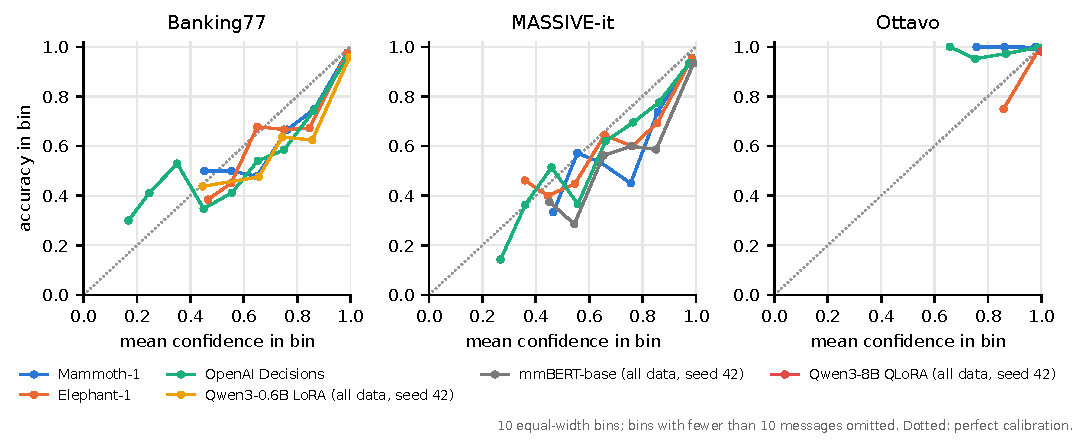
\includegraphics[width=\linewidth]{reliability.pdf}
\caption{Reliability diagrams on the historical test samples (decision models zero-shot with descriptions; best compact classifier
trained on all data, seed 42).}
\label{fig:reliability}
\end{figure}

\begin{figure}[t]
\centering
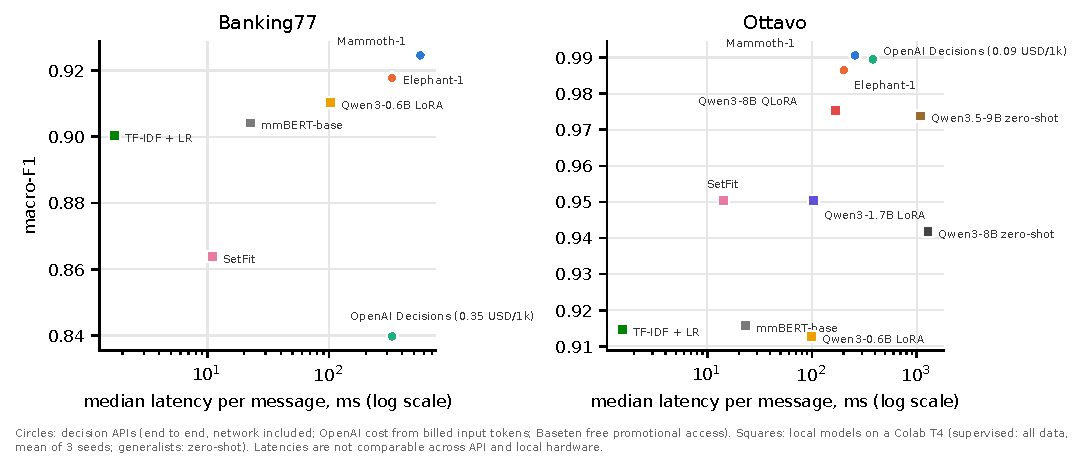
\includegraphics[width=\linewidth]{quality_latency.pdf}
\caption{Quality against median latency per message. API latencies include the network; local latencies were measured on a Colab T4;
the two are not comparable as hardware measurements.}
\label{fig:quality}
\end{figure}

\begin{table}[t]
\centering\small
\caption{Cost elements with their basis. Measured values come from this study; the labelling rate is an explicit assumption. No
break-even volume is reported because it depends on labelling and infrastructure costs that were not measured.}
\label{tab:costs}
\resizebox{\linewidth}{!}{\begin{tabular}{lrrr}
\toprule
Item & Ottavo-like (24 classes) & Banking77-like (77 classes) & Basis \\
\midrule
OpenAI Decisions{,} zero-shot{,} USD per 1M messages & 91 & 349 & measured (beta price) \\
Elephant-1 / Mammoth-1{,} USD per 1M messages & n/a & n/a & promotional access{,} no price \\
Labels for 20 per class & 480 & 1{,}540 & protocol \\
Labels for the full training sets used here & 1{,}669 & 9{,}993 & protocol \\
Person-hours to label 20 per class (one annotator) & 4 & 13 & assumption: 120 labels/hour \\
Person-hours to label the full sets (one annotator) & 14 & 83 & assumption: 120 labels/hour \\
mmBERT-base: training on all Ottavo data{,} T4 minutes & 2 & -- & measured \\
mmBERT-base: inference{,} T4 GPU-hours per 1M messages & 6.5 & -- & upper bound from batch-1 latency \\
Qwen3-0.6B LoRA: training on all Ottavo data{,} T4 minutes & 5 & -- & measured \\
Qwen3-0.6B LoRA: inference{,} T4 GPU-hours per 1M messages & 27.5 & -- & upper bound from batch-1 latency \\
Qwen3-8B QLoRA: training on all Ottavo data{,} T4 minutes & 51 & -- & measured \\
Qwen3-8B QLoRA: inference{,} T4 GPU-hours per 1M messages & 46.2 & -- & upper bound from batch-1 latency \\
\bottomrule
\end{tabular}}
\end{table}

\begin{figure}[t]
\centering
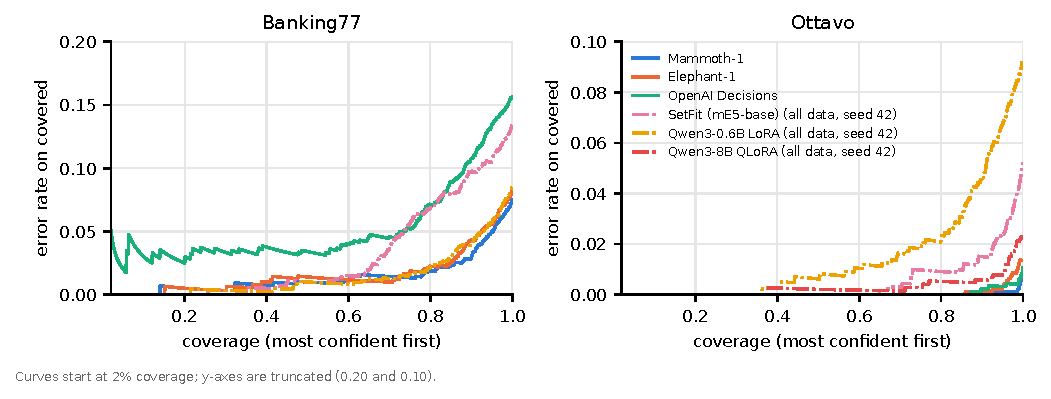
\includegraphics[width=\linewidth]{risk_coverage.pdf}
\caption{Risk--coverage curves: error rate among the most confident predictions as coverage grows.}
\label{fig:risk}
\end{figure}

\begin{table}[t]
\centering\footnotesize
\caption{Automatic acceptance with cross-fitted thresholds (decision models zero-shot with descriptions). $n$: test messages, each
evaluated once per run on the half not used to choose its threshold. Coverage: share of predictions accepted (range over runs in
parentheses). Err./acc.: errors and accepted predictions, summed over runs. Error: observed error among accepted predictions, with a 95\% bootstrap interval that
resamples messages and keeps all runs of a message together (2{,}000 replicates). Refused requests count as sent to review.}
\label{tab:selective}
\setlength{\tabcolsep}{4pt}
\begin{tabular}{llrrrrrl}
\toprule
Data & System & Target & $n$ & Runs & Coverage & Err./acc. & Error [95\% CI] \\
\midrule
Banking77 & Mammoth-1 & 2\% & 1000 & 1 & 84\% & 20 / 841 & 2.4\% [1.4, 3.4] \\
 & Elephant-1 & 2\% & 1000 & 1 & 79\% & 16 / 794 & 2.0\% [1.1, 3.0] \\
 & OpenAI Decisions & 2\% & 1000 & 1 & 0\% & 0 / 0 & -- \\
 & Qwen3-0.6B, all data & 2\% & 1000 & 3 & 80\% (78--83) & 49 / 2388 & 2.1\% [1.4, 2.9] \\
 & Qwen3-0.6B, expl. recipe & 2\% & 1000 & 4 & 89\% (87--91) & 69 / 3554 & 1.9\% [1.3, 2.7] \\
 & Mammoth-1 & 5\% & 1000 & 1 & 95\% & 48 / 953 & 5.0\% [3.7, 6.5] \\
 & Elephant-1 & 5\% & 1000 & 1 & 92\% & 45 / 925 & 4.9\% [3.5, 6.4] \\
 & OpenAI Decisions & 5\% & 1000 & 1 & 68\% & 32 / 677 & 4.7\% [3.2, 6.4] \\
 & Qwen3-0.6B, all data & 5\% & 1000 & 3 & 93\% (93--94) & 143 / 2800 & 5.1\% [4.1, 6.3] \\
 & Qwen3-0.6B, expl. recipe & 5\% & 1000 & 4 & 97\% (97--98) & 195 / 3894 & 5.0\% [4.0, 6.2] \\
\midrule
MASSIVE-it & Mammoth-1 & 2\% & 996 & 1 & 39\% & 7 / 388 & 1.8\% [0.5, 3.3] \\
 & Elephant-1 & 2\% & 996 & 1 & 25\% & 7 / 246 & 2.8\% [0.9, 5.1] \\
 & OpenAI Decisions & 2\% & 996 & 1 & 21\% & 12 / 213 & 5.6\% [2.7, 9.1] \\
 & mmBERT-base, all data & 2\% & 996 & 3 & 38\% (30--42) & 28 / 1130 & 2.5\% [1.4, 3.6] \\
 & Mammoth-1 & 5\% & 996 & 1 & 83\% & 38 / 823 & 4.6\% [3.3, 6.1] \\
 & Elephant-1 & 5\% & 996 & 1 & 77\% & 40 / 771 & 5.2\% [3.7, 6.8] \\
 & OpenAI Decisions & 5\% & 996 & 1 & 33\% & 20 / 333 & 6.0\% [3.6, 8.8] \\
 & mmBERT-base, all data & 5\% & 996 & 3 & 67\% (63--70) & 112 / 2012 & 5.6\% [4.3, 7.0] \\
\midrule
Ottavo & Mammoth-1 & 2\% & 960 & 1 & 100\% & 7 / 958 & 0.7\% [0.3, 1.3] \\
 & Elephant-1 & 2\% & 960 & 1 & 100\% & 13 / 959 & 1.4\% [0.6, 2.1] \\
 & OpenAI Decisions & 2\% & 960 & 1 & 100\% & 8 / 958 & 0.8\% [0.3, 1.5] \\
 & Qwen3-8B, all data & 2\% & 960 & 3 & 98\% (97--99) & 58 / 2834 & 2.0\% [1.5, 2.7] \\
 & Mammoth-1 & 5\% & 960 & 1 & 100\% & 7 / 958 & 0.7\% [0.3, 1.3] \\
 & Elephant-1 & 5\% & 960 & 1 & 100\% & 13 / 959 & 1.4\% [0.6, 2.1] \\
 & OpenAI Decisions & 5\% & 960 & 1 & 100\% & 8 / 958 & 0.8\% [0.3, 1.5] \\
 & Qwen3-8B, all data & 5\% & 960 & 3 & 100\% (100--100) & 70 / 2874 & 2.4\% [1.8, 3.2] \\
\bottomrule
\end{tabular}
\end{table}
